%% =====================================================================
%% HCAN-CIB manuscript -- Elsevier CAS single-column (cas-sc)
%% Needs cas-sc.cls and cas-common.sty in the project (use Overleaf's
%% "Elsevier CAS Single Column" template and replace its main .tex with this).
%% Text in RED, e.g. [verify: ...], marks values missing from the supplied
%% files. Delete the \vrf{} wrappers once resolved.
%% =====================================================================
\documentclass[a4paper,fleqn]{cas-sc}

\usepackage{amsmath,amssymb,amsfonts,bm}
\usepackage{booktabs,array,multirow}
\usepackage{xcolor}
\usepackage{tikz}
\usetikzlibrary{positioning,arrows.meta,calc}
\usepackage{algorithm}
\usepackage{algpseudocode}

\graphicspath{{figures/}}
\newcommand{\vrf}[1]{\textcolor{red}{[verify: #1]}}
\newcommand{\pmsd}[2]{$#1\pm#2$}
\DeclareMathOperator{\softmax}{softmax}
\DeclareMathOperator{\Var}{Var}
\DeclareMathOperator{\AUROC}{AUROC}
\newtheorem{proposition}{Proposition}
\newproof{pf}{Proof}

\begin{document}
\let\WriteBookmarks\relax
\def\floatpagefraction{0.8}
\def\textpagefraction{0.001}

\shorttitle{Invariance-gated multimodal emotion recognition under LOSO}
\shortauthors{First Author et al.}

\begin{highlights}
\item Leakage-free LOSO benchmark over 55 subjects on DEAP and DREAMER
\item Subject identity carries 349.6 times more variance than the emotion label
\item Invariance gates up-weight frontal and suppress EMG-prone temporal regions
\item Z-scoring and latent DeepSMOTE lift DREAMER AUROC from 0.478 to 0.559
\item A shallow linear model on Z-scored DE features still beats all deep models on DEAP
\end{highlights}

\title [mode = title]{Resolving Modality Starvation and Latent Class Collapse in Cross-Subject Multimodal Emotion Recognition: A Hierarchical Invariance-Gated Architecture}

\author[1]{First Author}[orcid=0000-0000-0000-0000]
\cormark[1]
\ead{first.author@university.edu}
\credit{Conceptualization, Methodology, Software, Formal analysis, Writing -- original draft}

\author[1]{Second Author}
\credit{Methodology, Validation, Writing -- review \& editing}

\author[1]{Supervisor Name}
\credit{Supervision, Writing -- review \& editing}

\affiliation[1]{organization={Department of Computer Science and Engineering, University Name},
  city={City},
  country={Country}}

\cortext[cor1]{Corresponding author}

\begin{abstract}
Emotion recognition from electroencephalography (EEG) and peripheral physiology is routinely reported at 75--85\% accuracy, yet most of those figures come from evaluation protocols in which windows of a single recording appear on both sides of the train/test boundary. Under a strict, leakage-free leave-one-subject-out (LOSO) protocol the picture changes sharply: three widely used deep baselines (EEGNet, ACRNN, a plain 1D-CNN) land between 0.49 and 0.54 AUROC on both DEAP (32 subjects) and DREAMER (23 subjects). We trace this failure to three interacting causes: biased, majority-leaning predictions at the level of individual held-out subjects, gradient starvation between modalities and channels, and an inter-subject variance that is $349.6\times$ larger than the emotion-label variance in DEAP differential-entropy features. We propose HCAN-CIB, a Hierarchical Cross-Attention Network with Channel and Modality Invariance Balancing. It combines per-channel temporal encoders, region-grouped fusion with an L2 spectral-decoupling penalty, an EMA-driven invariance gate that re-weights cortical regions by their cross-subject stability, transductive per-subject Z-scoring, and DeepSMOTE oversampling in the latent space. On DREAMER, the full pipeline moves AUROC from $0.4783\pm0.1395$ (base HCAN-CIB) to $0.5381\pm0.1567$ with Z-scoring and to $0.5589\pm0.1638$ with DeepSMOTE, turns the Gini coefficient positive ($+0.1178$), and lowers expected calibration error to $0.2249$ among HCAN-CIB variants. On DEAP, latent oversampling raises the minority prediction rate of HCAN-CIB from $0.499$ to $0.538$ and the minority recall to $0.540$, but a shallow logistic regression on Z-scored differential-entropy features still reaches $0.5754\pm0.0991$ AUROC and outperforms every deep model. Diagnostics show that learned embeddings remain organised by subject rather than by emotion. We therefore position inter-subject domain shift, not class imbalance or modality imbalance, as the remaining bottleneck, and we release a leakage-free benchmark across 55 subjects as a reference point for future work.
\end{abstract}

\begin{keywords}
Emotion recognition \sep EEG \sep multimodal fusion \sep leave-one-subject-out \sep gradient starvation \sep spectral decoupling \sep DeepSMOTE \sep domain shift
\end{keywords}

\maketitle

\section{Introduction}
\label{sec:intro}

Affective computing aims to infer a person's emotional state from signals the person does not consciously control. Scalp EEG reflects cortical activity that is directly tied to appraisal and valence processing, while peripheral channels such as electrocardiography (ECG), galvanic skin response, and respiration capture the autonomic side of the same episode. Combining the two is attractive because each modality is partially blind where the other is informative: autonomic signals respond slowly and non-specifically, whereas EEG is fast but dominated by noise and by anatomy.

A usable system must work on a person it has never seen. That requirement makes leave-one-subject-out (LOSO) validation the only protocol with clinical meaning: every trial, window, and normalisation statistic that touches the held-out person must be excluded from training and model selection. Many published pipelines do not satisfy this requirement. Random splits over overlapping windows, or subject-dependent 10-fold schemes, allow the network to see near-duplicates of test segments during training, and the reported accuracy then measures memorisation of a recording rather than recognition of an emotion \citep{li2022tutorial}.

We build a strictly leakage-free LOSO pipeline for DEAP \citep{koelstra2012deap} and DREAMER \citep{katsigiannis2018dreamer} and ask why deep multimodal models fail under it. Our experiments isolate three obstacles.

\begin{enumerate}
\item \textbf{Biased predictions at the subject level.} Each person uses the rating scale differently, so the binary labels of a held-out subject can be skewed, and models that minimise cross-entropy drift toward the more frequent class. On DEAP, EEGNet predicts the minority class for only $29.1\%$ of windows; its Macro-F1 is $0.4005$.
\item \textbf{Modality and channel starvation.} When a high-dimensional EEG stream is fused with a low-dimensional peripheral vector, the branch with the steeper initial loss descent captures the gradient budget and the other branch is barely trained \citep{pezeshki2021gradient,wang2020makes}.
\item \textbf{Inter-subject variance.} In DEAP differential-entropy (DE) features, subject identity explains $47.75\%$ of the variance and the emotion label explains $0.137\%$, a ratio of $349.6{:}1$. Subject identity can be decoded with $97.81\%$ accuracy, against a chance level of $3.125\%$.
\end{enumerate}

Our contributions are as follows.
\begin{itemize}
\item We give a systematic, quantitative diagnosis of majority-leaning prediction, gradient starvation, and subject variance in multimodal LOSO affective computing, and we test each cause with a dedicated intervention.
\item We propose HCAN-CIB, which combines channel-independent 1D feature extraction, region-grouped spectral decoupling, and an EMA-based invariance gate that re-weights cortical regions according to their cross-subject stability.
\item We integrate DeepSMOTE oversampling in the latent embedding space, which raises minority recall without synthesising artifact-laden raw time series.
\item We report a leakage-free benchmark over 55 subjects (32 DEAP and 23 DREAMER) with paired non-parametric tests, calibration metrics, and interpretability analyses, including a negative result: a shallow linear model on normalised DE features beats all deep models on DEAP.
\end{itemize}

The rest of the paper is organised as follows. Section~\ref{sec:related} reviews related work, Section~\ref{sec:method} presents HCAN-CIB, Section~\ref{sec:setup} describes the experimental protocol, Section~\ref{sec:results} reports and discusses results, and Section~\ref{sec:conclusion} concludes.

%% ---------------------------------------------------------------------
\section{Literature Survey}
\label{sec:related}

\subsection{Deep architectures for EEG emotion recognition}
Compact convolutional networks dominate current practice. EEGNet couples temporal convolutions with depthwise spatial filters and has far fewer parameters than earlier CNNs \citep{lawhern2018eegnet}. ACRNN adds channel-wise attention and self-attention on top of a convolutional--recurrent stack and reports strong results on DEAP \citep{tao2020acrnn}. Frequency-domain alternatives, built on DE features extracted from standard bands, are common on the SEED family of datasets \citep{duan2013de,zheng2015seed}. A recent review catalogues these designs and highlights the heterogeneity of evaluation protocols across papers \citep{li2022tutorial}. A shared design choice in the convolutional models is early spatial mixing: the depthwise spatial kernel collapses all electrodes into a handful of virtual channels before any region-specific structure is learned.

\subsection{Multimodal fusion and gradient starvation}
Joint training of several modalities frequently underperforms the best unimodal model, because the branches overfit and generalise at different rates \citep{wang2020makes}. Subsequent work attributes the effect to modality competition and proposes on-the-fly gradient modulation to slow the dominant branch \citep{peng2022balanced,huang2022modality}. Gradient starvation provides a more general account: once a feature allows the loss to fall quickly, the gradient signal for slower features shrinks toward zero. Spectral decoupling, a penalty on the magnitude of the network output, counteracts this effect by keeping the loss from saturating on the dominant feature \citep{pezeshki2021gradient}. We adapt that idea to intermediate representations and make it region-aware.

\subsection{Class imbalance and domain adaptation in physiological computing}
SMOTE interpolates between minority neighbours in input space \citep{chawla2002smote}, which is hazardous for raw EEG because linear blends of two waveforms generally do not resemble real brain activity. Generative approaches such as GAMO operate on learned features \citep{mullick2019gamo}, and DeepSMOTE performs SMOTE-style interpolation inside the latent space of an autoencoder \citep{dablain2023deepsmote}. For subject shift, domain-adversarial training removes domain identity from the features through a gradient reversal layer \citep{ganin2016dann}, and bi-hemispheric variants have been applied to EEG emotion recognition \citep{li2021bidann}.

\subsection{Gap}
Three observations motivate this work. First, evaluation protocols that leak windows across the split inflate reported accuracy. Second, imbalance remedies and modality-balancing remedies are usually proposed and evaluated separately, so their individual contributions to cross-subject performance remain confounded. Third, the effect of subject-level amplitude offsets is seldom quantified. Our study evaluates all three factors under one leakage-free protocol and with matched metrics.

%% ---------------------------------------------------------------------
\section{Methodology}
\label{sec:method}

\subsection{Problem statement}
Let $\mathcal{D}=\{\mathcal{S}_1,\dots,\mathcal{S}_K\}$ be a collection of $K$ subjects, where $\mathcal{S}_k=\{(\mathbf{X}^{\mathrm{eeg}}_{k,i},\mathbf{X}^{\mathrm{per}}_{k,i},y_{k,i})\}_{i=1}^{n_k}$. Each EEG window satisfies $\mathbf{X}^{\mathrm{eeg}}\in\mathbb{R}^{C\times T}$, with $C$ electrodes and $T$ samples. The peripheral recording $\mathbf{X}^{\mathrm{per}}\in\mathbb{R}^{P\times T'}$ is reduced by a fixed statistical descriptor map to a vector $\mathbf{p}\in\mathbb{R}^{d_p}$ with $d_p=24$ for DEAP and $d_p=12$ for DREAMER. The label $y\in\{0,1\}$ is the binarised valence class. In fold $k$, the model is fitted on $\mathcal{D}\setminus\mathcal{S}_k$ and evaluated only on $\mathcal{S}_k$:
\begin{equation}
\theta_k^\star=\arg\min_{\theta}\;\mathbb{E}_{(\mathbf{X},y)\sim\mathcal{D}\setminus\mathcal{S}_k}\,\ell\bigl(f_\theta(\mathbf{X}),y\bigr),\qquad
\text{score}_k=M\bigl(f_{\theta_k^\star},\mathcal{S}_k\bigr).
\end{equation}

\subsection{Transductive per-subject Z-scoring}
Scalp impedance, skull thickness, and resting alpha power shift the amplitude distribution of every person. For subject $s$, channel $c$, we compute the mean $\mu_{s,c}$ and standard deviation $\sigma_{s,c}$ over all samples of that subject's recording and set
\begin{equation}
\tilde{x}_{s,c,t}=\frac{x_{s,c,t}-\mu_{s,c}}{\sigma_{s,c}+10^{-8}}.\label{eq:z}
\end{equation}
The statistics use no labels, but they use the unlabeled recording of the test subject, so the step is transductive. In deployment it requires a short calibration recording of the new user. The same normalisation is applied to the ECG and peripheral inputs.

\subsection{Overview}
Figure~\ref{fig:arch} shows the data flow for DEAP. The EEG branch is processed by channel-independent encoders (Stage~A), aggregated into regional tokens by intra-region attention (Stage~C), and re-weighted by the invariance gate (Stage~B). The peripheral branch yields a single query token. Cross-modal attention fuses the two, DeepSMOTE operates on the fused embedding during training only, and a linear head produces the logit.

\begin{figure}[t]
\centering
\resizebox{\textwidth}{!}{%
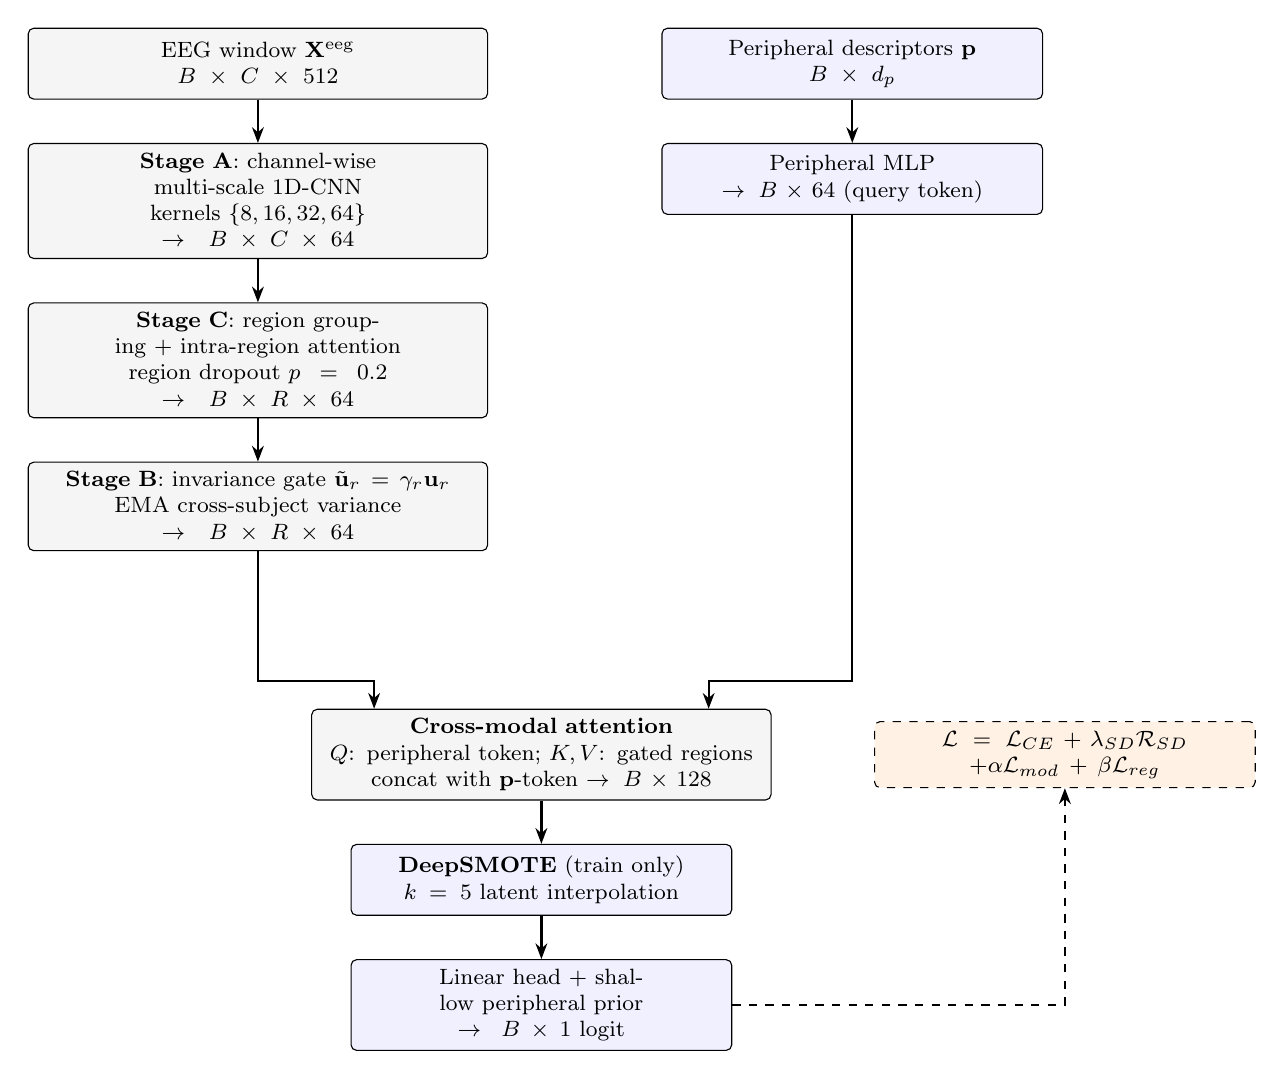
\begin{tikzpicture}[
  node distance=0.55cm,
  blk/.style={draw,rounded corners=2pt,align=center,font=\footnotesize,minimum height=0.9cm,text width=5.6cm,fill=gray!8},
  sm/.style={draw,rounded corners=2pt,align=center,font=\footnotesize,minimum height=0.9cm,text width=4.6cm,fill=blue!6},
  loss/.style={draw,dashed,rounded corners=2pt,align=center,font=\footnotesize,text width=4.6cm,fill=orange!10},
  arr/.style={-{Stealth[length=2mm]},thick}]
\node[blk] (eeg) {EEG window $\mathbf{X}^{\mathrm{eeg}}$\\$B\times C\times 512$};
\node[blk,below=of eeg] (sa) {\textbf{Stage A}: channel-wise multi-scale 1D-CNN\\kernels $\{8,16,32,64\}$\\$\to B\times C\times 64$};
\node[blk,below=of sa] (sc) {\textbf{Stage C}: region grouping + intra-region attention\\region dropout $p=0.2$\\$\to B\times R\times 64$};
\node[blk,below=of sc] (sb) {\textbf{Stage B}: invariance gate $\tilde{\mathbf{u}}_r=\gamma_r\mathbf{u}_r$\\EMA cross-subject variance\\$\to B\times R\times 64$};
\node[sm,right=2.2cm of eeg] (per) {Peripheral descriptors $\mathbf{p}$\\$B\times d_p$};
\node[sm,below=of per] (mlp) {Peripheral MLP\\$\to B\times 64$ (query token)};
\node[blk,below=2.0cm of sb,xshift=3.6cm] (xa) {\textbf{Cross-modal attention}\\$Q$: peripheral token; $K,V$: gated regions\\concat with $\mathbf{p}$-token $\to B\times128$};
\node[sm,below=of xa] (ds) {\textbf{DeepSMOTE} (train only)\\$k=5$ latent interpolation};
\node[sm,below=of ds] (hd) {Linear head $+$ shallow peripheral prior\\$\to B\times1$ logit};
\node[loss,right=1.3cm of xa] (ls) {$\mathcal{L}=\mathcal{L}_{CE}+\lambda_{SD}\mathcal{R}_{SD}$\\$+\alpha\mathcal{L}_{mod}+\beta\mathcal{L}_{reg}$};
\draw[arr] (eeg)--(sa); \draw[arr] (sa)--(sc); \draw[arr] (sc)--(sb);
\draw[arr] (per)--(mlp);
\draw[arr] (sb.south) |- ($(xa.north west)+(0.8,0.35)$) -- ($(xa.north west)+(0.8,0)$);
\draw[arr] (mlp.south) |- ($(xa.north east)+(-0.8,0.35)$) -- ($(xa.north east)+(-0.8,0)$);
\draw[arr] (xa)--(ds); \draw[arr] (ds)--(hd);
\draw[arr,dashed] (hd.east) -| (ls.south);
\end{tikzpicture}}
\caption{HCAN-CIB data flow for DEAP ($C=32$, $R=5$, $d_p=24$). For DREAMER, $C=14$, $R=4$ and $d_p=12$. $B$ denotes batch size. Dashed elements are training-time only.}
\label{fig:arch}
\end{figure}

\subsection{Stage A: channel-independent temporal encoders}
Standard depthwise spatial convolutions merge all electrodes in a single learned kernel, which couples the gradient of every channel to that of the loudest channel. Stage~A avoids early spatial mixing. Each electrode signal $\mathbf{x}_c\in\mathbb{R}^{T}$ is passed through its own temporal encoder $\phi_c$ built from parallel 1D convolutions with kernel sizes $k\in\{8,16,32,64\}$, which cover gamma bursts as well as theta and alpha rhythms:
\begin{equation}
\mathbf{h}_c=\mathbf{W}_h\Bigl[\,\mathrm{GAP}\bigl(\sigma(\mathrm{BN}(\mathbf{w}^{(k)}_c * \mathbf{x}_c))\bigr)\,\Bigr]_{k\in\{8,16,32,64\}}\in\mathbb{R}^{d},\qquad d=64,
\end{equation}
where $*$ is 1D convolution, $\mathrm{GAP}$ is global average pooling over time, and $\sigma$ is a ReLU-type nonlinearity \vrf{confirm activation and whether encoder weights are shared across channels or fully separate}. The output of Stage~A is the token set $\{\mathbf{h}_c\}_{c=1}^{C}$.

\subsection{Stage C: region grouping and spectral decoupling}
Electrodes are partitioned into $R$ cortical regions $\mathcal{G}_1,\dots,\mathcal{G}_R$: five regions in DEAP (frontal, temporal, central, parietal, occipital) and four in DREAMER (frontal, temporal, central, parietal), because the 14-channel Emotiv montage has no dedicated occipital group \vrf{list the electrode-to-region assignment}. Intra-region attention produces one token per region:
\begin{equation}
a_c=\frac{\exp\bigl(\mathbf{v}_r^{\top}\tanh(\mathbf{W}_r\mathbf{h}_c)\bigr)}{\sum_{c'\in\mathcal{G}_r}\exp\bigl(\mathbf{v}_r^{\top}\tanh(\mathbf{W}_r\mathbf{h}_{c'})\bigr)},\qquad
\mathbf{u}_r=\sum_{c\in\mathcal{G}_r}a_c\,\mathbf{h}_c.
\end{equation}
During training, entire regions are dropped with probability $0.2$ to prevent reliance on a single area.

\paragraph{Spectral-decoupling regulariser.}
Let $\mathbf{z}_{\mathrm{eeg}}$ and $\mathbf{z}_{\mathrm{per}}$ denote the pooled EEG and peripheral representations. The total objective is
\begin{equation}
\mathcal{L}_{\mathrm{total}}=\mathcal{L}_{CE}+\lambda_{SD}\,\mathcal{R}_{SD}+\alpha\,\mathcal{L}_{\mathrm{mod}}+\beta\,\mathcal{L}_{\mathrm{reg}},
\label{eq:total}
\end{equation}
with
\begin{equation}
\mathcal{R}_{SD}=\sum_{r=1}^{R}\frac{1}{\gamma_r}\,\|\mathbf{u}_r\|_2^2+\|\mathbf{z}_{\mathrm{per}}\|_2^2 .
\label{eq:sd}
\end{equation}
Here $\mathcal{L}_{\mathrm{mod}}$ is an auxiliary cross-entropy on each modality-specific head, $\mathcal{L}_{\mathrm{reg}}$ is an auxiliary cross-entropy on each regional token, and $(\lambda_{SD},\alpha,\beta)=(0.001,0.3,0.2)$. The factor $1/\gamma_r$ couples the penalty to Stage~B: regions judged unstable receive a heavier norm penalty. Setting $\gamma_r\equiv1$ and $\mathbf{u}_r$ pooled recovers the plain two-term form $\lambda_{SD}(\|\mathbf{z}_{\mathrm{eeg}}\|_2^2+\|\mathbf{z}_{\mathrm{per}}\|_2^2)$.

\begin{proposition}[Norm bound]
Let a binary logistic head $f=\mathbf{w}^{\top}\mathbf{z}$ be trained with $\mathcal{L}=\mathrm{CE}(\sigma(f),y)+\lambda\|\mathbf{z}\|_2^2$. Any stationary point in $\mathbf{z}$ satisfies $\|\mathbf{z}\|_2=|\sigma(f)-y|\,\|\mathbf{w}\|_2/(2\lambda)<\|\mathbf{w}\|_2/(2\lambda)$.
\end{proposition}
\begin{pf}
Setting $\nabla_{\mathbf{z}}\mathcal{L}=(\sigma(f)-y)\mathbf{w}+2\lambda\mathbf{z}=\mathbf{0}$ gives $\mathbf{z}=-(\sigma(f)-y)\mathbf{w}/(2\lambda)$, and $|\sigma(f)-y|<1$ for finite $f$.
\end{pf}
The bound illustrates the mechanism. Without the penalty, a representation that separates the training set can grow without limit, its cross-entropy gradient vanishes, and any slower branch stops receiving a useful learning signal. With the penalty, the dominant branch cannot saturate the loss, so the gradient budget stays available to the other branch. The statement is exact for a linear head; for the full network it is a motivating argument rather than a guarantee.

\paragraph{Cross-modal fusion.}
The peripheral token $\mathbf{q}=\mathrm{MLP}(\mathbf{p})$ acts as the query over the gated region tokens $\tilde{\mathbf{U}}=[\tilde{\mathbf{u}}_1;\dots;\tilde{\mathbf{u}}_R]$:
\begin{equation}
\mathbf{m}=\softmax\!\left(\frac{(\mathbf{W}_Q\mathbf{q})(\mathbf{W}_K\tilde{\mathbf{U}})^{\top}}{\sqrt{d}}\right)\mathbf{W}_V\tilde{\mathbf{U}},\qquad
\mathbf{z}=[\mathbf{m};\mathbf{q}]\in\mathbb{R}^{128}.
\end{equation}
A residual shallow prior adds $\mathbf{w}_s^{\top}\mathbf{p}$ to the final logit, so that the fused model cannot do worse than a linear peripheral classifier.

\subsection{Stage B: dynamic invariance gating}
Stage~B estimates, for every region, how consistently it helps across training subjects. Let $\ell_{r,s}$ be the auxiliary cross-entropy of region $r$ on the batch share of subject $s$. An exponential moving average maintains
\begin{equation}
m_{r,s}\leftarrow\rho\,m_{r,s}+(1-\rho)\,\ell_{r,s},\qquad
v_r=\Var_{s}\bigl(m_{r,s}\bigr),\qquad
g_r=\frac{1}{v_r+\epsilon},
\end{equation}
and the gate coefficient is normalised to have unit mean over regions,
\begin{equation}
\gamma_r=R\,\frac{g_r}{\sum_{r'=1}^{R}g_{r'}},\qquad \tilde{\mathbf{u}}_r=\gamma_r\,\mathbf{u}_r .
\end{equation}
A region whose loss contribution varies strongly between people, for example the temporal electrodes close to the masseter and temporalis muscles, receives $\gamma_r<1$. A region with stable contribution receives $\gamma_r>1$. Because $\gamma_r$ also enters Eq.~\eqref{eq:sd}, suppressed regions are simultaneously attenuated in the forward pass and penalised in norm. The EMA decay $\rho$ and the numerical constant $\epsilon$ follow the repository defaults \vrf{insert $\rho$, $\epsilon$, any clipping range on $\gamma_r$}.

\subsection{Stage D: DeepSMOTE in the latent space}
Interpolating raw EEG windows produces waveforms with no physiological counterpart. We instead oversample the fused embedding $\mathbf{z}$. A lightweight autoencoder with decoder $\mathcal{D}$ is trained jointly with a reconstruction term
\begin{equation}
\mathcal{L}_{\mathrm{rec}}=\|\mathcal{D}(\mathbf{z})-\mathbf{z}_{\mathrm{target}}\|_2^2 ,
\end{equation}
which keeps the embedding geometry smooth \vrf{state the exact reconstruction target and the weight of $\mathcal{L}_{\mathrm{rec}}$}. For each minority embedding $\mathbf{z}_i$, one of its $k=5$ minority nearest neighbours $\mathbf{z}_{nn}$ is drawn and a synthetic code is created,
\begin{equation}
\mathbf{z}_{\mathrm{syn}}=\mathbf{z}_i+\lambda\,(\mathbf{z}_{nn}-\mathbf{z}_i),\qquad \lambda\sim\mathcal{U}(0,1),
\end{equation}
until the two classes have equal size in the batch. Synthetic codes are passed to the classification head and are used during training only. The held-out subject is never oversampled. For comparison, V-SMOTE applies the same interpolation without the autoencoder, and GAMO generates minority embeddings adversarially.

\subsection{Algorithm}
Algorithm~\ref{alg:loso} summarises training and model selection under LOSO.

\begin{algorithm}[t]
\caption{HCAN-CIB training and LOSO model selection}
\label{alg:loso}
\begin{algorithmic}[1]
\Require Subjects $\mathcal{D}=\{\mathcal{S}_1,\dots,\mathcal{S}_K\}$; hyperparameters $\lambda_{SD},\alpha,\beta,\rho,k$
\For{$k=1$ \textbf{to} $K$}
  \State $\mathcal{S}_{\mathrm{test}}\gets\mathcal{S}_k$;\; draw 4 subjects from $\mathcal{D}\setminus\mathcal{S}_k$ as $\mathcal{S}_{\mathrm{val}}$;\; $\mathcal{S}_{\mathrm{tr}}\gets$ remaining subjects
  \State Z-score each subject independently (Eq.~\ref{eq:z}); window the recordings
  \State Initialise $\theta$, EMA states $m_{r,s}$, gates $\gamma_r\gets1$
  \For{each epoch}
    \For{each mini-batch from $\mathcal{S}_{\mathrm{tr}}$}
      \State Compute $\mathbf{h}_c$ (Stage A), $\mathbf{u}_r$ (Stage C), $\mathbf{q}$
      \State Update $m_{r,s}$, $v_r$, $\gamma_r$ (Stage B); form $\tilde{\mathbf{u}}_r=\gamma_r\mathbf{u}_r$
      \State $\mathbf{z}\gets$ cross-modal attention$(\mathbf{q},\tilde{\mathbf{U}})$
      \State \textbf{if} DeepSMOTE \textbf{then} append $\mathbf{z}_{\mathrm{syn}}$ until classes are balanced
      \State Evaluate $\mathcal{L}_{\mathrm{total}}$ (Eq.~\ref{eq:total}) and take an optimiser step
    \EndFor
    \State Compute validation AUROC on $\mathcal{S}_{\mathrm{val}}$; early-stop on it
  \EndFor
  \State Choose the decision threshold $\tau_k$ on $\mathcal{S}_{\mathrm{val}}$ only
  \State Evaluate the best checkpoint on $\mathcal{S}_{\mathrm{test}}$ with threshold $\tau_k$; store all metrics and the gates $\gamma_r$
\EndFor
\State \Return mean and standard deviation of every metric over the $K$ folds
\end{algorithmic}
\end{algorithm}

%% ---------------------------------------------------------------------
\section{Experimental Setup}
\label{sec:setup}

\subsection{Datasets}
\textbf{DEAP} \citep{koelstra2012deap} contains 32 subjects with 40 one-minute music-video trials each. We use the 32 EEG channels sampled at 128~Hz and the 8 peripheral channels. Recordings are cut into 4~s windows (512 samples) with 2~s overlap. Valence ratings are binarised by a per-subject median split, which makes labels nearly balanced (mean positive rate $0.4977$, range $0.450$--$0.500$; no subject has a majority class above $70\%$).

\noindent\textbf{DREAMER} \citep{katsigiannis2018dreamer} contains 23 subjects who watched 18 audio-visual clips. We use the 14 EEG channels of the Emotiv EPOC (128~Hz) and 2 ECG channels (256~Hz), the latter summarised into 12 statistical features. Windowing and the valence binarisation rule follow the repository defaults \vrf{state DREAMER window length/overlap and the rating threshold used for binarisation}.

\subsection{Baselines}
\textbf{EEGNet} \citep{lawhern2018eegnet} applies a temporal convolution, a depthwise spatial convolution, and a separable convolution, followed by a linear classifier. \textbf{ACRNN} \citep{tao2020acrnn} uses a convolutional front end with channel-wise attention, a recurrent layer, and self-attention. \textbf{PlainCNN} is a stack of 1D convolutions with global pooling. All three consume EEG only. A fourth reference, a shallow \textbf{logistic regression} on Z-scored DE features in four frequency bands ($32\times4=128$ dimensions) concatenated with peripheral descriptors, bounds what a linear model can extract.

\subsection{Evaluation protocol and metrics}
We run strict LOSO ($K=32$ on DEAP, $K=23$ on DREAMER). In each fold, four training subjects form an inner validation set that controls early stopping and the decision threshold; no information from the test subject enters training, selection, or thresholding, apart from the label-free normalisation statistics of Section~\ref{sec:method}. We report accuracy, balanced accuracy \citep{brodersen2010balanced}, AUROC, the Gini coefficient $2\,\AUROC-1$, PR-AUC \citep{saito2015pr}, Macro-F1, the Matthews correlation coefficient (MCC) \citep{chicco2020mcc}, $\Delta_{\mathrm{trivial}}$ (accuracy minus the accuracy of always predicting the majority class), minority-class recall, minority prediction rate (the share of windows assigned to the minority class), and expected calibration error (ECE) \citep{guo2017calibration} computed with \vrf{number and type of bins}. Values are means $\pm$ standard deviations over folds. Paired comparisons across folds use the Wilcoxon signed-rank test \citep{wilcoxon1945} with Holm correction \citep{holm1979}.

\subsection{Implementation details}
Optimiser, learning rate, batch size, epoch budget, and random seeds are taken from the configuration files of the repository \vrf{fill in optimiser, learning rate, batch size, max epochs, early-stopping patience, seeds, hardware}. The hyperparameters of Eq.~\eqref{eq:total} are $\lambda_{SD}=0.001$, $\alpha=0.3$, $\beta=0.2$ for every HCAN-CIB variant.

\subsection{Latent visualisation protocol}
Test-fold embeddings are projected to two dimensions with t-SNE \citep{vandermaaten2008tsne} using perplexity $30$, learning rate $200$, and $1000$ iterations.

%% ---------------------------------------------------------------------
\section{Results and Discussion}
\label{sec:results}

\subsection{Diagnosing the failure of cross-subject transfer}
Table~\ref{tab:diag} reports the variance diagnostics on DEAP DE features. Subject identity accounts for $349.6$ times more variance than the emotion label, and a simple classifier recovers the subject from the raw features with $97.81\%$ accuracy. After per-subject Z-scoring, that accuracy drops to $3.125\%$, which is chance. In the same step, the AUROC of a shallow logistic regression rises from $0.517\pm0.016$ ($p=0.112$ against chance) to $0.575\pm0.018$ ($p=0.0006$); the uncertainties here are standard errors over 32 folds. A linear model on EEG alone reaches $0.558$ ($p=0.003$). Cross-subject emotion information is present in the signal, and a large part of it is hidden behind subject-specific offsets.

\begin{table}[t]
\centering
\caption{Domain-shift diagnostics on DEAP differential-entropy features (32 subjects).}
\label{tab:diag}
\small
\begin{tabular}{lcc}
\toprule
Quantity & Raw DE features & Per-subject Z-scored \\
\midrule
Variance explained by subject, $\eta^2_{\mathrm{subj}}$ & $47.75\%$ & -- \\
Variance explained by label, $\eta^2_{\mathrm{label}}$ & $0.137\%$ & -- \\
Ratio $\eta^2_{\mathrm{subj}}/\eta^2_{\mathrm{label}}$ & $349.6$ & -- \\
Subject-identity decoding accuracy (chance $3.125\%$) & $97.81\%$ & $3.125\%$ \\
Shallow LR AUROC (mean $\pm$ SE) & $0.517\pm0.016$ & $0.575\pm0.018$ \\
$p$-value vs.\ chance & $0.112$ & $0.0006$ \\
\bottomrule
\end{tabular}
\end{table}

\subsection{Main benchmarks}
Tables~\ref{tab:dreamer1}--\ref{tab:deap2} list every metric for every pipeline. Two readings stand out. On DEAP, no deep pipeline exceeds $0.541$ AUROC, whereas the shallow linear model reaches $0.5754$. On DREAMER, the AUROC of the three baselines lies between $0.488$ and $0.517$, and only the GAMO, Z-scored, and DeepSMOTE variants of HCAN-CIB exceed $0.53$.

\begin{table}[t]
\centering
\caption{DREAMER, LOSO over 23 subjects: discrimination metrics (mean $\pm$ SD over folds). Bold marks the best value among all pipelines in the column.}
\label{tab:dreamer1}
\scriptsize
\resizebox{\textwidth}{!}{%
\begin{tabular}{lccccccc}
\toprule
Pipeline & Acc. & Bal. Acc. & AUROC & Gini & PR-AUC & Macro-F1 & MCC \\
\midrule
ACRNN & \pmsd{0.5362}{0.1243} & \pmsd{0.5137}{0.1032} & \pmsd{0.5169}{0.1242} & \pmsd{0.0338}{0.2484} & \pmsd{0.4799}{0.1590} & $\mathbf{0.4569\pm0.1256}$ & \pmsd{0.0202}{0.2337} \\
PlainCNN & \pmsd{0.5459}{0.1387} & \pmsd{0.4744}{0.0962} & \pmsd{0.4879}{0.1313} & \pmsd{-0.0242}{0.2625} & \pmsd{0.4627}{0.1469} & \pmsd{0.4104}{0.1123} & \pmsd{-0.0431}{0.2170} \\
EEGNet & $\mathbf{0.5990\pm0.0955}$ & \pmsd{0.4855}{0.1299} & \pmsd{0.4945}{0.1593} & \pmsd{-0.0110}{0.3187} & \pmsd{0.5015}{0.1586} & \pmsd{0.4452}{0.1403} & \pmsd{-0.0312}{0.2718} \\
HCAN-CIB (base) & \pmsd{0.4758}{0.1398} & \pmsd{0.4961}{0.0405} & \pmsd{0.4783}{0.1395} & \pmsd{-0.0434}{0.2791} & \pmsd{0.4493}{0.1731} & \pmsd{0.3546}{0.1000} & \pmsd{-0.0174}{0.1115} \\
HCAN-CIB (V-SMOTE) & \pmsd{0.5604}{0.1380} & \pmsd{0.5108}{0.0803} & \pmsd{0.5006}{0.1812} & \pmsd{0.0011}{0.3624} & \pmsd{0.4728}{0.1848} & \pmsd{0.3682}{0.1210} & \pmsd{0.0254}{0.1682} \\
HCAN-CIB (GAMO) & \pmsd{0.4372}{0.1344} & $\mathbf{0.5167\pm0.1003}$ & \pmsd{0.5331}{0.1729} & \pmsd{0.0663}{0.3459} & $\mathbf{0.5237\pm0.1501}$ & \pmsd{0.3875}{0.1508} & $\mathbf{0.0398\pm0.2049}$ \\
HCAN-CIB (Z-score) & \pmsd{0.5435}{0.1320} & \pmsd{0.5122}{0.0935} & \pmsd{0.5381}{0.1567} & \pmsd{0.0763}{0.3133} & \pmsd{0.5008}{0.1049} & \pmsd{0.4188}{0.1306} & \pmsd{0.0254}{0.2127} \\
HCAN-CIB (DeepSMOTE) & \pmsd{0.5580}{0.1375} & \pmsd{0.5105}{0.0849} & $\mathbf{0.5589\pm0.1638}$ & $\mathbf{0.1178\pm0.3276}$ & \pmsd{0.5125}{0.1270} & \pmsd{0.4166}{0.1244} & \pmsd{0.0182}{0.1812} \\
\bottomrule
\end{tabular}}
\end{table}

\begin{table}[t]
\centering
\caption{DREAMER: class-behaviour and calibration metrics. A negative $\Delta_{\mathrm{trivial}}$ means the model is less accurate than always predicting the majority class.}
\label{tab:dreamer2}
\small
\begin{tabular}{lcccc}
\toprule
Pipeline & $\Delta_{\mathrm{trivial}}$ & Minority recall & ECE & Minority pred. rate \\
\midrule
ACRNN & \pmsd{-0.0894}{0.1435} & \pmsd{0.5325}{0.3260} & \pmsd{0.2794}{0.1554} & \pmsd{0.5169}{0.2629} \\
PlainCNN & \pmsd{-0.0797}{0.1473} & \pmsd{0.4496}{0.3409} & \pmsd{0.3058}{0.1686} & \pmsd{0.4831}{0.3127} \\
EEGNet & \pmsd{-0.0266}{0.0693} & \pmsd{0.4266}{0.2959} & $\mathbf{0.1856\pm0.0806}$ & \pmsd{0.4469}{0.2540} \\
HCAN-CIB (base) & \pmsd{-0.1498}{0.1617} & \pmsd{0.6111}{0.4329} & \pmsd{0.2479}{0.1576} & \pmsd{0.6159}{0.4134} \\
HCAN-CIB (V-SMOTE) & \pmsd{-0.0652}{0.1406} & \pmsd{0.6180}{0.4493} & \pmsd{0.2514}{0.1329} & \pmsd{0.6039}{0.4357} \\
HCAN-CIB (GAMO) & \pmsd{-0.1884}{0.1685} & \pmsd{0.6385}{0.4010} & \pmsd{0.3244}{0.1436} & \pmsd{0.6184}{0.4004} \\
HCAN-CIB (Z-score) & \pmsd{-0.0821}{0.1225} & \pmsd{0.6189}{0.3642} & \pmsd{0.2371}{0.1033} & \pmsd{0.6014}{0.3380} \\
HCAN-CIB (DeepSMOTE) & \pmsd{-0.0676}{0.1236} & \pmsd{0.6193}{0.3419} & \pmsd{0.2249}{0.1030} & \pmsd{0.6014}{0.3263} \\
\bottomrule
\end{tabular}
\end{table}

\begin{table}[t]
\centering
\caption{DEAP, LOSO over 32 subjects: discrimination metrics (mean $\pm$ SD over folds). DeepSMOTE was evaluated on DREAMER only.}
\label{tab:deap1}
\scriptsize
\resizebox{\textwidth}{!}{%
\begin{tabular}{lccccccc}
\toprule
Pipeline & Acc. & Bal. Acc. & AUROC & Gini & PR-AUC & Macro-F1 & MCC \\
\midrule
ACRNN & \pmsd{0.5203}{0.0521} & \pmsd{0.5097}{0.0432} & \pmsd{0.5159}{0.0945} & \pmsd{0.0318}{0.1891} & \pmsd{0.5586}{0.0866} & \pmsd{0.4111}{0.0804} & \pmsd{0.0285}{0.1268} \\
CNN & \pmsd{0.5070}{0.0538} & \pmsd{0.5122}{0.0449} & \pmsd{0.5407}{0.0851} & \pmsd{0.0814}{0.1702} & \pmsd{0.5649}{0.0858} & \pmsd{0.4117}{0.0896} & \pmsd{0.0335}{0.1254} \\
EEGNet & \pmsd{0.5141}{0.0484} & \pmsd{0.5002}{0.0412} & \pmsd{0.5220}{0.1069} & \pmsd{0.0440}{0.2138} & \pmsd{0.5442}{0.0835} & \pmsd{0.4005}{0.0834} & \pmsd{-0.0021}{0.1201} \\
HCAN-CIB (raw) & \pmsd{0.5063}{0.0723} & \pmsd{0.5147}{0.0715} & \pmsd{0.5148}{0.0911} & \pmsd{0.0295}{0.1822} & \pmsd{0.5533}{0.0705} & \pmsd{0.4825}{0.0823} & \pmsd{0.0378}{0.1585} \\
HCAN-CIB (V-SMOTE) & \pmsd{0.5109}{0.0658} & \pmsd{0.5029}{0.0646} & \pmsd{0.5138}{0.0809} & \pmsd{0.0276}{0.1618} & \pmsd{0.5433}{0.0625} & \pmsd{0.4704}{0.0881} & \pmsd{-0.0026}{0.1544} \\
HCAN-CIB (GAMO) & \pmsd{0.5016}{0.0750} & \pmsd{0.4927}{0.0685} & \pmsd{0.5011}{0.0876} & \pmsd{0.0022}{0.1752} & \pmsd{0.5445}{0.0677} & \pmsd{0.4433}{0.0932} & \pmsd{-0.0278}{0.1619} \\
HCAN-CIB (Z-score) & \pmsd{0.5156}{0.0792} & \pmsd{0.5163}{0.0799} & \pmsd{0.5298}{0.1129} & \pmsd{0.0597}{0.2259} & \pmsd{0.5519}{0.0979} & \pmsd{0.5042}{0.0845} & \pmsd{0.0332}{0.1712} \\
Shallow LR (DE + Z) & $\mathbf{0.5539\pm0.0617}$ & $\mathbf{0.5539\pm0.0617}$ & $\mathbf{0.5754\pm0.0991}$ & $\mathbf{0.1508\pm0.1982}$ & $\mathbf{0.5947\pm0.0901}$ & $\mathbf{0.5501\pm0.0640}$ & $\mathbf{0.1118\pm0.1246}$ \\
\bottomrule
\end{tabular}}
\end{table}

\begin{table}[t]
\centering
\caption{DEAP: class-behaviour and calibration metrics.}
\label{tab:deap2}
\small
\begin{tabular}{lcccc}
\toprule
Pipeline & $\Delta_{\mathrm{trivial}}$ & Minority recall & ECE & Minority pred. rate \\
\midrule
ACRNN & \pmsd{0.0180}{0.0512} & \pmsd{0.3645}{0.3583} & \pmsd{0.2302}{0.1461} & \pmsd{0.3547}{0.3720} \\
CNN & \pmsd{0.0047}{0.0506} & \pmsd{0.4187}{0.3874} & \pmsd{0.2508}{0.1497} & \pmsd{0.4062}{0.3887} \\
EEGNet & \pmsd{0.0117}{0.0504} & \pmsd{0.2910}{0.3398} & $\mathbf{0.1733\pm0.1018}$ & \pmsd{0.2906}{0.3329} \\
HCAN-CIB (raw) & \pmsd{0.0039}{0.0721} & \pmsd{0.5142}{0.2430} & \pmsd{0.3319}{0.1034} & \pmsd{0.4992}{0.2389} \\
HCAN-CIB (V-SMOTE) & \pmsd{0.0086}{0.0657} & \pmsd{0.5404}{0.2244} & \pmsd{0.3280}{0.0936} & \pmsd{0.5375}{0.2272} \\
HCAN-CIB (GAMO) & \pmsd{-0.0008}{0.0727} & \pmsd{0.4767}{0.2943} & \pmsd{0.3550}{0.1065} & \pmsd{0.4836}{0.2820} \\
HCAN-CIB (Z-score) & \pmsd{0.0133}{0.0793} & \pmsd{0.5298}{0.1730} & \pmsd{0.4023}{0.0963} & \pmsd{0.5133}{0.1513} \\
Shallow LR (DE + Z) & $\mathbf{0.0539\pm0.0617}$ & $\mathbf{0.5641\pm0.1342}$ & \pmsd{0.2458}{0.0366} & \pmsd{0.5078}{0.0827} \\
\bottomrule
\end{tabular}
\end{table}

\subsection{Majority-leaning predictions and latent oversampling}
On DEAP the labels are nearly balanced by construction, so low minority prediction rates reflect a bias of the learned decision function rather than a skewed training set. EEGNet assigns only $29.1\%$ of windows to the minority class (recall $0.291$), and ACRNN assigns $35.5\%$. HCAN-CIB without oversampling already rises to $0.499$, and V-SMOTE brings the minority prediction rate to $0.538$ with a minority recall of $0.540$ (Table~\ref{tab:deap2}). Macro-F1 of HCAN-CIB (raw) is $0.4825$ against $0.4005$ for EEGNet. The change in class behaviour is real, but AUROC does not follow it ($0.5148\to0.5138$ with V-SMOTE and $0.5011$ with GAMO). A balanced decision rule is therefore a necessary condition for fair evaluation, not a sufficient condition for generalisation.

On DREAMER, the minority prediction rate of every HCAN-CIB variant sits near $0.60$--$0.62$ and the minority recall near $0.61$--$0.64$, compared with $0.43$--$0.53$ recall for the baselines. These variants over-assign the minority class slightly, which lowers accuracy below the trivial majority rule (negative $\Delta_{\mathrm{trivial}}$ in Table~\ref{tab:dreamer2}), and this is also why the Macro-F1 of HCAN-CIB variants stays below that of ACRNN ($0.4569$). Within the HCAN-CIB family, DeepSMOTE attains the highest AUROC ($0.5589$) and Gini ($+0.1178$) and the lowest ECE ($0.2249$), while the Z-score variant has a marginally higher Macro-F1 ($0.4188$ versus $0.4166$). EEGNet remains better calibrated in absolute terms ($0.1856$).

\subsection{Normalisation and oversampling ablation on DREAMER}
Table~\ref{tab:ablation} traces the progression. Adding Z-scoring raises AUROC from $0.4783$ to $0.5381$ ($+0.0598$) and Gini from $-0.0434$ to $+0.0763$. Adding DeepSMOTE on top of Z-scoring raises AUROC to $0.5589$ ($+0.0208$), for a total gain of $+0.0806$ over the base model. The Macro-F1 gain is concentrated in the normalisation step ($0.3546\to0.4188$); DeepSMOTE leaves it essentially unchanged. We stress that fold-level standard deviations ($0.14$--$0.16$ AUROC) exceed these gains, and that we did not run a paired test between the DREAMER variants. The ordering is consistent, but the individual increments should be read as modest effects, not as established differences.

\begin{table}[t]
\centering
\caption{Stepwise ablation of HCAN-CIB on DREAMER.}
\label{tab:ablation}
\small
\begin{tabular}{lcccc}
\toprule
Configuration & AUROC & Gini & Macro-F1 & ECE \\
\midrule
Base HCAN-CIB (raw) & \pmsd{0.4783}{0.1395} & $-0.0434$ & \pmsd{0.3546}{0.1000} & \pmsd{0.2479}{0.1576} \\
\; $+$ per-subject Z-score & \pmsd{0.5381}{0.1567} & $+0.0763$ & \pmsd{0.4188}{0.1306} & \pmsd{0.2371}{0.1033} \\
\; $+$ DeepSMOTE (latent) & \pmsd{0.5589}{0.1638} & $+0.1178$ & \pmsd{0.4166}{0.1244} & \pmsd{0.2249}{0.1030} \\
\midrule
Absolute change, base $\to$ full & $+0.0806$ & $+0.1612$ & $+0.0620$ & $-0.0230$ \\
\bottomrule
\end{tabular}
\end{table}

\subsection{Modality starvation}\label{sec:starv}
All three baselines are EEG-only, so they cannot show whether the peripheral stream contributes. HCAN-CIB includes the peripheral branch, the shallow peripheral prior, and the spectral-decoupling penalty of Eq.~\eqref{eq:sd}, and Proposition~1 shows how the penalty limits the norm of a dominant representation. The empirical test of the starvation hypothesis is indirect: if modality imbalance were the primary cause of failure, balancing it should lift cross-subject AUROC. It did not. On DEAP, EEG-only baselines ($0.516$--$0.541$) and the balanced multimodal HCAN-CIB ($0.515$) differ by less than one fold-level standard deviation. We conclude that modality starvation is a real design hazard that our architecture addresses, but not the factor that limits cross-subject accuracy in these datasets. A direct measurement, for instance per-branch gradient norms and unimodal ablations of the trained model, is not part of the present experiments and would make this claim testable at the mechanism level \vrf{add unimodal/gradient-norm experiment if available}.

\subsection{Invariance-gate interpretability}
Figure~\ref{fig:gates} shows the regional gates across the 23 DREAMER folds, and Table~\ref{tab:gates} lists their statistics. Under Z-scoring, the frontal gate averages $1.193\pm0.161$ (maximum $1.481$ in fold 19), the parietal gate $1.085\pm0.211$, the central gate $0.874\pm0.172$, and the temporal gate $0.849\pm0.149$ (minimum $0.456$ in fold 1). With DeepSMOTE the pattern is the same: frontal $1.139\pm0.155$, parietal $1.104\pm0.217$, temporal $0.831\pm0.136$. This ranking agrees with two physiological expectations. Frontal asymmetry is a well-documented correlate of valence, and temporal electrodes sit next to the jaw and temporal muscles, whose electromyographic activity is idiosyncratic and broadband. The gate learned to suppress exactly the region with the highest expected artefact load, without being told which region that is. The empty occipital column in the DREAMER heat maps reflects that DREAMER defines only four regions.

The gate pattern is not universal. In the DEAP run reported in the repository, the gates came out as temporal $1.125\pm0.310$, parietal $1.050\pm0.300$, central $1.019\pm0.207$, occipital $0.991\pm0.269$, and frontal $0.815\pm0.283$ \vrf{confirm which DEAP configuration produced these gate values}. Here the frontal region is attenuated, consistent with the ocular blink artefacts that dominate frontal channels in DEAP, and the temporal region is boosted, in line with the auditory character of the music-video stimuli. The two datasets differ in stimulus modality, hardware, and electrode count, and the gate adapts accordingly. We note that gates alone did not lift AUROC beyond $0.60$ on raw signals; they are an interpretability and regularisation mechanism, and not a remedy for subject shift.

\begin{figure}[t]
\centering
\begin{minipage}{0.49\textwidth}
\centering
\includegraphics[width=\linewidth]{gate_heatmap_dreamer_zscore.png}\\
{\small (a) Z-score}
\end{minipage}\hfill
\begin{minipage}{0.49\textwidth}
\centering
\includegraphics[width=\linewidth]{gate_heatmap_dreamer_deepsmote.png}\\
{\small (b) DeepSMOTE}
\end{minipage}
\caption{Stage~B region invariance gates $\gamma_r$ for each of the 23 held-out DREAMER subjects. Frontal and parietal regions are consistently up-weighted; the temporal region is down-weighted.}
\label{fig:gates}
\end{figure}

\begin{table}[t]
\centering
\caption{Mean $\pm$ SD of Stage~B gate values across held-out folds (DREAMER).}
\label{tab:gates}
\small
\begin{tabular}{lcc}
\toprule
Region & Z-score & DeepSMOTE \\
\midrule
Frontal & \pmsd{1.193}{0.161} & \pmsd{1.139}{0.155} \\
Parietal & \pmsd{1.085}{0.211} & \pmsd{1.104}{0.217} \\
Central & \pmsd{0.874}{0.172} & \vrf{value} \\
Temporal & \pmsd{0.849}{0.149} & \pmsd{0.831}{0.136} \\
\bottomrule
\end{tabular}
\end{table}

\subsection{Latent geometry and residual domain shift}
Figure~\ref{fig:tsne} shows t-SNE projections of the learned embeddings, coloured by class. Neither the Z-score model nor the DeepSMOTE model collapses to a single region of the latent space: points of both classes occupy the whole embedding. But the two classes are interleaved at every scale, and no region of the plot is dominated by one emotion. The embeddings form elongated, filament-like groups. We interpret this local structure as organisation by recording session or subject rather than by emotion, which fits the $349.6{:}1$ variance ratio and the finding that subject identity is almost perfectly decodable. We have not yet verified this interpretation with a subject-coloured projection or a quantitative metric such as a silhouette score by subject; this check should accompany the figure in the final version \vrf{add subject-coloured t-SNE or subject-vs-class silhouette}. Latent oversampling therefore cures the lopsided decision behaviour but leaves the dominant source of variation untouched.

\begin{figure}[t]
\centering
\begin{minipage}{0.49\textwidth}
\centering
\includegraphics[width=\linewidth]{tsne_brain_embeddings_dreamer_zscore.png}\\
{\small (a) Z-score}
\end{minipage}\hfill
\begin{minipage}{0.49\textwidth}
\centering
\includegraphics[width=\linewidth]{tsne_brain_embeddings_dreamer_deepsmote.png}\\
{\small (b) DeepSMOTE}
\end{minipage}
\caption{t-SNE of DREAMER embeddings coloured by class (perplexity 30, learning rate 200, 1000 iterations). Class labels are interleaved, so the learned space does not separate valence classes for unseen subjects.}
\label{fig:tsne}
\end{figure}

\subsection{Deep raw-waveform models versus a linear floor}
Each EEG window of DEAP holds $32\times512=16{,}384$ values dominated by phase offsets and subject-specific waveform detail. With 31 training subjects, a convolutional network can lower training loss by memorising those subject signatures. The symptom on unseen subjects is over-confidence: HCAN-CIB (Z-score) has an ECE of $0.4023$ and a Brier score of $0.406$, worse than the $0.250$ of an uninformative constant predictor, whereas the shallow model has an ECE of $0.2458$. Band-limited DE features summarise power in four frequency bands, discard phase, and, after Z-scoring, remove the subject offset. A linear model on these features reaches $0.5754\pm0.0991$ AUROC.

Table~\ref{tab:wilcoxon} gives the paired comparisons over the 32 DEAP folds. The difference to HCAN-CIB (raw) is significant after Holm correction ($p_{\mathrm{adj}}=0.040$). The differences to HCAN-CIB (Z-score), EEGNet, and PlainCNN are of similar size ($-0.034$ to $-0.053$) but do not reach significance after correction ($p_{\mathrm{adj}}\ge0.192$). The accurate statement is that the linear model is nominally best and significantly better than one of four deep alternatives, and that the study has limited power with 32 folds and fold-level SDs near $0.10$. The AUROC of the shallow model against chance, in contrast, is clearly significant ($p=0.0006$).

\begin{table}[t]
\centering
\caption{Paired Wilcoxon signed-rank tests against the shallow LR reference on DEAP (AUROC; mean $\pm$ SE over 32 folds; Holm correction over the four comparisons).}
\label{tab:wilcoxon}
\small
\begin{tabular}{lcccc}
\toprule
Model & AUROC & Diff.\ vs.\ ref. & Wilcoxon $p$ & Holm $p_{\mathrm{adj}}$ \\
\midrule
Shallow LR (DE + Z) & \pmsd{0.575}{0.018} & -- & -- & -- \\
HCAN-CIB (Z-score) & \pmsd{0.530}{0.020} & $-0.045$ & $0.064$ & $0.192$ \\
PlainCNN & \pmsd{0.541}{0.015} & $-0.034$ & $0.200$ & $0.200$ \\
EEGNet & \pmsd{0.522}{0.019} & $-0.053$ & $0.076$ & $0.192$ \\
HCAN-CIB (raw) & \pmsd{0.515}{0.016} & $-0.060$ & $0.010$ & $0.040$ \\
\bottomrule
\end{tabular}
\end{table}

\subsection{Limitations}
First, absolute performance is low. The best AUROC is $0.5589$ on DREAMER and the best deep result on DEAP is $0.541$, and with fold-level SDs of $0.09$--$0.16$ the confidence intervals of neighbouring pipelines overlap. Second, DeepSMOTE was evaluated on DREAMER only, and no paired tests were run among DREAMER variants. Third, the Z-scoring step is transductive and assumes access to unlabeled data from the new user. Fourth, the starvation analysis is indirect (Section~\ref{sec:starv}). Fifth, only valence was analysed; arousal is left to future work. Finally, we did not explore different DEAP label thresholds, subject-specific calibration, or post-hoc probability calibration such as temperature scaling.

%% ---------------------------------------------------------------------
\section{Conclusion}
\label{sec:conclusion}

Under a strict leakage-free LOSO protocol on 55 subjects, widely used deep EEG models perform close to chance, and the apparent progress reported in the literature depends on how the split is built. We separated three candidate causes and tested an intervention for each. Latent oversampling repairs minority-class behaviour (DEAP minority prediction rate $0.29\to0.54$ for the best oversampled variant against EEGNet; DREAMER minority recall $\approx0.62$). Spectral decoupling and cross-modal attention address modality starvation by design. Per-subject Z-scoring and DeepSMOTE together lift DREAMER AUROC from $0.4783$ to $0.5589$ and lower the calibration error among HCAN-CIB variants. None of these steps, however, removes the dominant source of error: embeddings stay organised by person, and a linear model on normalised DE features ($0.5754$ AUROC) still beats all deep models on DEAP.

Two directions follow directly from the evidence. The first is to feed Z-scored DE band features into the cross-attention backbone, replacing the raw-waveform encoders, so that the deep model starts from the linear floor instead of from 16{,}384 raw values per window. The second is subject-adversarial domain adaptation (Stage~E), with a gradient reversal layer and a subject discriminator attached to the fused embedding \citep{ganin2016dann}, together with post-hoc probability calibration. We expect the combination to be the most direct route past the current ceiling, and the leakage-free benchmark in this paper provides the baseline against which such gains can be measured.

\section*{Declaration of competing interest}
The authors declare that they have no known competing financial interests or personal relationships that could have influenced the work reported in this paper.

\section*{Data and code availability}
DEAP and DREAMER are available from their original distributors. Code and fold-level results: \vrf{GitHub URL}.

%% ---------------------------------------------------------------------
%% References (numeric). Verify every entry against the publisher record
%% before submission (volume, pages, DOI).
\begin{thebibliography}{99}
\bibitem{koelstra2012deap} S.~Koelstra, C.~Muhl, M.~Soleymani, J.-S. Lee, A.~Yazdani, T.~Ebrahimi, T.~Pun, A.~Nijholt, I.~Patras, DEAP: A database for emotion analysis using physiological signals, IEEE Trans.\ Affect.\ Comput.\ 3~(1) (2012) 18--31.
\bibitem{katsigiannis2018dreamer} S.~Katsigiannis, N.~Ramzan, DREAMER: A database for emotion recognition through EEG and ECG signals from wireless low-cost off-the-shelf devices, IEEE J.\ Biomed.\ Health Inform.\ 22~(1) (2018) 98--107.
\bibitem{lawhern2018eegnet} V.~J. Lawhern, A.~J. Solon, N.~R. Waytowich, S.~M. Gordon, C.~P. Hung, B.~J. Lance, EEGNet: A compact convolutional neural network for EEG-based brain--computer interfaces, J.\ Neural Eng.\ 15~(5) (2018) 056013.
\bibitem{tao2020acrnn} W.~Tao, C.~Li, R.~Song, J.~Cheng, Y.~Liu, F.~Wan, X.~Chen, EEG-based emotion recognition via channel-wise attention and self attention, IEEE Trans.\ Affect.\ Comput.\ 14~(1) (2023) 382--393.
\bibitem{pezeshki2021gradient} M.~Pezeshki, S.-O. Kaba, Y.~Bengio, A.~Courville, D.~Precup, G.~Lajoie, Gradient starvation: A learning proclivity in neural networks, in: Advances in Neural Information Processing Systems, volume~34, 2021, pp. 1256--1272.
\bibitem{wang2020makes} W.~Wang, D.~Tran, M.~Feiszli, What makes training multi-modal classification networks hard?, in: Proc.\ IEEE/CVF Conf.\ Computer Vision and Pattern Recognition, 2020, pp. 12695--12705.
\bibitem{peng2022balanced} X.~Peng, Y.~Wei, A.~Deng, D.~Wang, D.~Hu, Balanced multimodal learning via on-the-fly gradient modulation, in: Proc.\ IEEE/CVF Conf.\ Computer Vision and Pattern Recognition, 2022, pp. 8238--8247.
\bibitem{huang2022modality} Y.~Huang, J.~Lin, C.~Zhou, H.~Yang, L.~Huang, Modality competition: What makes joint training of multi-modal network fail in deep learning? (Provably), in: Proc.\ Int.\ Conf.\ Machine Learning, PMLR 162, 2022, pp. 9226--9259.
\bibitem{dablain2023deepsmote} D.~Dablain, B.~Krawczyk, N.~V. Chawla, DeepSMOTE: Fusing deep learning and SMOTE for imbalanced data, IEEE Trans.\ Neural Netw.\ Learn.\ Syst.\ 34~(9) (2023) 6390--6404.
\bibitem{chawla2002smote} N.~V. Chawla, K.~W. Bowyer, L.~O. Hall, W.~P. Kegelmeyer, SMOTE: Synthetic minority over-sampling technique, J.\ Artif.\ Intell.\ Res.\ 16 (2002) 321--357.
\bibitem{mullick2019gamo} S.~S. Mullick, S.~Datta, S.~Das, Generative adversarial minority oversampling, in: Proc.\ IEEE/CVF Int.\ Conf.\ Computer Vision, 2019, pp. 1695--1704.
\bibitem{ganin2016dann} Y.~Ganin, E.~Ustinova, H.~Ajakan, P.~Germain, H.~Larochelle, F.~Laviolette, M.~Marchand, V.~Lempitsky, Domain-adversarial training of neural networks, J.\ Mach.\ Learn.\ Res.\ 17~(59) (2016) 1--35.
\bibitem{li2021bidann} Y.~Li, W.~Zheng, Y.~Zong, Z.~Cui, T.~Zhang, X.~Zhou, A bi-hemisphere domain adversarial neural network model for EEG emotion recognition, IEEE Trans.\ Affect.\ Comput.\ 12~(2) (2021) 494--504.
\bibitem{li2022tutorial} X.~Li, Y.~Zhang, P.~Tiwari, D.~Song, B.~Hu, M.~Yang, Z.~Zhao, N.~Kumar, P.~Marttinen, EEG based emotion recognition: A tutorial and review, ACM Comput.\ Surv.\ 55~(4) (2022) 79.
\bibitem{zheng2015seed} W.-L. Zheng, B.-L. Lu, Investigating critical frequency bands and channels for EEG-based emotion recognition with deep neural networks, IEEE Trans.\ Auton.\ Ment.\ Dev.\ 7~(3) (2015) 162--175.
\bibitem{duan2013de} R.-N. Duan, J.-Y. Zhu, B.-L. Lu, Differential entropy feature for EEG-based emotion classification, in: Proc.\ 6th Int.\ IEEE/EMBS Conf.\ Neural Engineering, 2013, pp. 81--84.
\bibitem{guo2017calibration} C.~Guo, G.~Pleiss, Y.~Sun, K.~Q. Weinberger, On calibration of modern neural networks, in: Proc.\ Int.\ Conf.\ Machine Learning, PMLR 70, 2017, pp. 1321--1330.
\bibitem{vandermaaten2008tsne} L.~van~der Maaten, G.~Hinton, Visualizing data using t-SNE, J.\ Mach.\ Learn.\ Res.\ 9 (2008) 2579--2605.
\bibitem{wilcoxon1945} F.~Wilcoxon, Individual comparisons by ranking methods, Biometrics Bull.\ 1~(6) (1945) 80--83.
\bibitem{holm1979} S.~Holm, A simple sequentially rejective multiple test procedure, Scand.\ J.\ Stat.\ 6~(2) (1979) 65--70.
\bibitem{brodersen2010balanced} K.~H. Brodersen, C.~S. Ong, K.~E. Stephan, J.~M. Buhmann, The balanced accuracy and its posterior distribution, in: Proc.\ 20th Int.\ Conf.\ Pattern Recognition, 2010, pp. 3121--3124.
\bibitem{saito2015pr} T.~Saito, M.~Rehmsmeier, The precision-recall plot is more informative than the ROC plot when evaluating binary classifiers on imbalanced datasets, PLoS ONE 10~(3) (2015) e0118432.
\bibitem{chicco2020mcc} D.~Chicco, G.~Jurman, The advantages of the Matthews correlation coefficient (MCC) over F1 score and accuracy in binary classification evaluation, BMC Genomics 21 (2020) 6.
\end{thebibliography}

\printcredits

\end{document}
